\chapter{Gamma Astronomy}

\section{The Field of Astroparticle Physics}

The ballon flights of Victor Hess \cite{Hess:1912srp} are
often times cited as the starting point of astroparticle physics,
because they gave reason to believe, that the measured ionizing
radiation is of extraterrestrial origin. 

The radiation was referenced as "Höhenstrahlung" 
(see e.g. \cite{myssowsky1926versuche}) 
and "cosmic rays" (see e.g. \cite{millikan1928origin}) with 
the english term cosmic rays eventually winning out.

Soon after, in 1933, Carl D. Anderson discovered the existence
of antimatter using a cloud chamber \cite{PhysRev.43.491},
which is crucial for the measurement of especially
high energy photons.

Later years brought the discovery of several new particles,
that are imperative to modern astronomy:
pions \cite{LATTES1947}, muons \cite{PhysRev.52.1003}
and neutrinos \cite{Cowan103}.

Recently, the so far last discovery on this journey
was made with the measurement of the first gravitational 
waves \cite{PhysRevLett.118.221101}.

This leaves the field of astronomy with four different
messengers, which coins the term
multi messenger astronomy:
\begin{enumerate}
	\item Electromagnetic radiation
	\item Cosmic rays
	\item Neutrinos
	\item Gravitational waves
\end{enumerate}

Figure \ref{fig:multi_messenger} illustrates the key differences between
photons, protons and neutrinos.

\begin{figure}
	\centering
	\captionsetup{width=0.9\linewidth}
	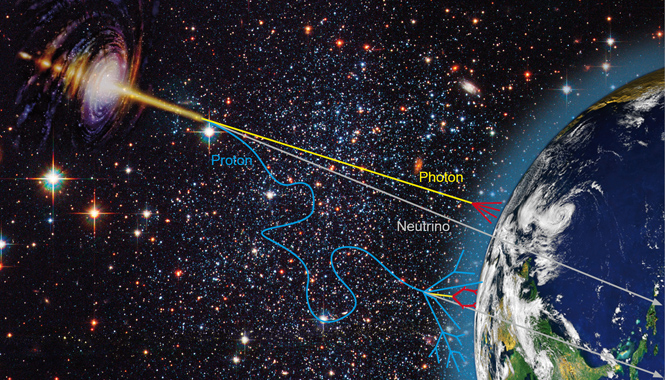
\includegraphics[width=0.9\textwidth]{images/astro-web-titel.jpg}
	\caption{Visualization of the behaviors of different messengers
		particles in modern astronomy.
		Photons and neutrinos travel through the universe without deflection,
		because they do not carry an electric charge.
		Neutrinos interact less than photons,
		which leads to a high proportion passing through earth.
		Charged cosmic rays get deflected by interstellar
		magnetic fields and thus generally do not allow for a reconstruction
		of the source position.
		The image is taken from the DESY-website at \cite{desy_mm_astro}.
	}
	\label{fig:multi_messenger}
\end{figure}


\section{Gamma Research}
In contrast to charged cosmic rays, $\gamma$-rays point towards
their sources, allowing to search for bright sources of radiation.
This makes it possible to learn more about the acceleration processes
and sources, that produce high energy gamma and cosmic rays.
Two important classes of proposed sources are active galactic nuclei,
which are considered massive black holes, that produce jets and 
supernove remnants. (mehr research)

Researching the diffuse component of gamma-rays on the other hand holds
potential to find out more about interstellar magnetic fields and the
propagation of relativistic particles in the universe.

Another motivation to research gamma-rays lies in the assumption, that
dark matter could annihilate to photon pairs. (quelle im tu netz öffnen)

Due to the way gamma-rays are being detected, it is not possible
to avoid measuring cosmic rays as well.
At the same time cosmic rays are much more numerous,
which makes them the dominant background in gamma astronomy \cite{funcray}.

\section{Production of Gamma-Rays}
Creation of high-energy gamma-rays can not happen thermally,
but happens in a combination of high energy charged particles 
and interstellar targets or magnetic fields \cite{funcray}.
A model for the production at the source, the Self Synchroton Comptoon model,
focuses on photon emission from an initial pure electron distribution.
The key aspects of this model are now briefly presented. 

\textbf{Synchroton Radiation}

Propposed sources of cosmic and gamma rays include 
high magnetic fields. Any moving charged particle will thus be
deflected perpendicular to its moving direction
due to the Lorentz-force, forcing them on a radial trajectory.
At the same time a relativistic charged particle, 
that gets accelerated radially, emits synchroton 
photons with average energy given by:

\begin{equation}
	\langle E_{\gamma} \rangle \propto \frac{1}{M_P} E_P^2 B^2.
	\label{eq:synchroton}
\end{equation}

Here, $M_P$ and $E_P$ denote the accelerated particle's 
mass and energy respectively. With the inverse mass dependency 
it is immediately evident that
synchroton radiation plays a major role in leptonic 
emission and much less in hadronic emission.

A direct result of this is, that the electrons energy gets reduced
in the process, affecting ("cooling") the initial electron distribution.
This is sometimes referred to as synchroton cooling.

The emitted synchroton spectrum needs to be further modified 
if the emitting region is optically thick and photons 
get absorbed by the medium.
This is in fact always the case, as the regions contains 
both magnetic fields and a high density of electrons.

\textbf{Inverse Compton Scattering}
In a classical particle interpretation photons and electrons 
can collide exchanging energy and altering their directions.
For the normal case of Compton scattering the electron 
is assumed to be at rest and the photon can never gain 
energy by colliding with the electron.
This can be 
seen by the increase in wavelength in \eqref{eq:compton},
with $\lambda^{\prime}$ denoting the scattered photons 
wavelength, $\lambda$ denoting the initial photons wavelength  
and $\Theta$ denoting the scattering angle.

\begin{equation}
	\lambda^{\prime} - \lambda  \propto \left(1-\cos{\Theta} \right)
	\label{eq:compton}
\end{equation}

If the electron itself is moving with much higher energy
than the photon, this changes and the photon can gain substantial energy.
This is reffered to as inverse Compton scattering.
In that case, transforming the equations to the 
electron's frame of reference and back to the laboratory frame of reference
boosts the photons energy by a factor $\gamma$ for each transformation, 
with $\gamma$ being the Lorentz factor of the electron.

A limit to the photon energies is set by the scattering cross
section, which reduces with higher photon energies.
For low energies the cross section can be approximated by 
the Thomson cross section, for high energies
one uses the Klein-Nishina cross section. (quellen angeben)

The Synchroton Self Compton model combines the above mentioned
effects to produce a photon energy distribution from an
electron distribution, which is often times assumed to
follow a power-law spectrum initially.
The free parameters of the model can be interpreted as 
three frequencies: The minimum injection frequency $\nu_m$, 
the cooling frequency $\nu_c$ and the self-absorption frequency $\nu_a$.
Depending on the order of these parameters, different 
photon distributions can be generated.

A detailed analysis of the influence of the parameters of
the Synchroton Self Compton model, can be found in 
\cite{10.1093/mnras/stt1461}.


\section{Types of experiments}
Emitted $\gamma$-rays can be observed either directly
from outside the atmosphere via satellites or indirectly
via ground based gamma astronomy.

The different types of experiments differ in the way particles are detected and
the resulting energy ranges, where they are most sensitive.

\subsection{Satellite Experiments}
Satellite experiments allow direct measurements of gamma and cosmic rays, because of the operation
above the atmosphere.
This allows to use similar techniques as experiments located at terrestrial 
particle detectors: Incoming photons hit an initial layer and produce an electron pair 
via pair production. The tracks of these particles get observed before they reach the calorimeter,
where their energies get measured.

Despite the advantages over ground based experiments, the small detector areas 
limit the sensitivities at higher energies.

A currently operating example is the FERMI Gamma-ray Space Observatory (FGST) \cite{Atwood_2009}.
The Large Area Telescope (LAT) on 
the FGST covers an energy range of
\SI{20}{\mega\electronvolt} to \SI{100}{\giga\electronvolt} \cite{Atwood_2009}.
It is able to cover a huge field ov view (fov) of 
\SI{20}{\degree}. A second detector, the Gamma-ray Burst Monitor,
searches for gamma ray bursts using a scintilator setup to notify other experiments.

\subsection{Imaging Air Cherenkov Telescopes}
A class of ground-based observatories are the 
Imaging Air Cherenkov Telescopes (IACTs),
which will be the focus of this thesis.

In constrast to the satellite experiments, they cannot directly
observe the cosmic particle. Instead they use the atmosphere as detector medium.
High energy primary particles generate a cascade of secondary particles
when interacting with the atmosphere. These particles generate cherenkov
light, which is recorded by the IACTs.

Modern experiments include 
MAGIC \cite{ALEKSIC2012435},
VERITAS \cite{WEEKES2002221}
and HESS \cite{vincent2005hess},
all of which consist of multiple telescopes to observe the shower 
from different angles to improve the reconstruction.

The observable energy range generally generally lies in the range of
some \SI{10}{\giga\electronvolt} to some 10-\SI{100}{\tera\electronvolt}.

\subsection{Air Shower Arrays}
Air shower arrays, like IACTs, operate on the ground and thus also have 
to measure the particle indirectly.

In contrast to IACT-experiments, air shower arrays consist of a huge
number of single scintillation detectors, spaced on a grid on the ground.
Instead of the cherenkov light, they measure the
remaining particles of the shower. This makes them feasible
for energies even above the ones measured by IACTs.

A modern experiment is the High Altitude Water Cherenkov Observatory (HAWC) \cite{2015ICRC...34..966S}.
It uses \num{300} water tanks to measure air showers with a lower threshold
of under \SI{1}{\tera\electronvolt}.

\section{Detection of Gamma Rays with IACTs}
\subsection{Measuring Events}
\label{sec:measuring}

The primary particles of gamma or cosmic rays cannot be 
observed with IACTs directly. Instead one can measure the secondary particles
that emerge from the particles interaction with matter.

If the primary particle energy is high enough, the resulting 
secondary particles can interact with the atmosphere themself, thus starting a 
cascade of secondary particles.
Particles, that have enough energy, are faster than the local speed of light.
Because the electrons carry a charge and the air acts as dielectricum, 
cherenkov light gets emitted \cite{smth}.

Cherenkov photons get collected by the mirror(s) of a telescope
and projected onto a camera system mounted above the mirror.
Figure \ref{fig:iact_mirror_camera} illustrates the measurement of 
an air shower.

\begin{figure}
	\centering
	\captionsetup{width=0.9\linewidth}
	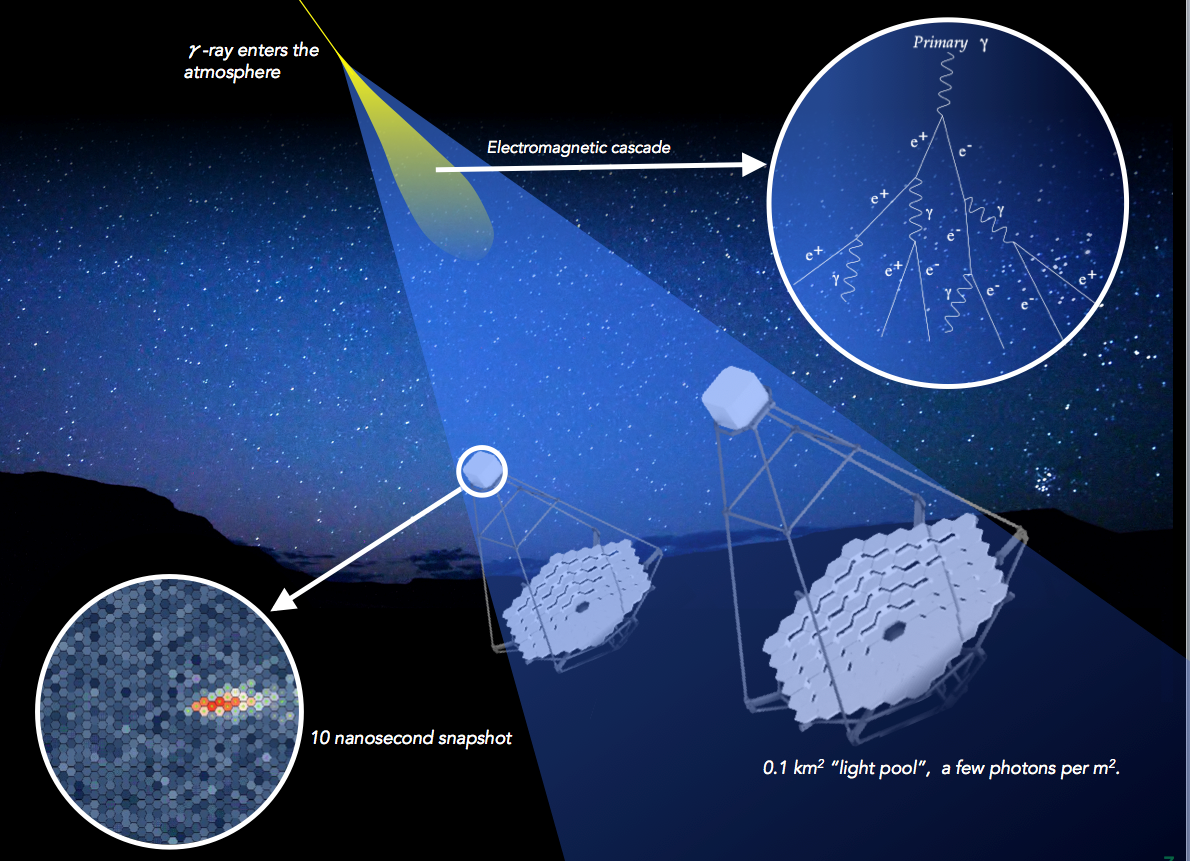
\includegraphics[width=0.9\textwidth]{images/cta47.png}
	\caption{A schematic illustration of the working principles of 
	an IACT experiment:
	A $\gamma$-ray produces an air shower in the atmosphere
	that points roughly towards the telescopes.
	Cherenkov light from the air shower 
	hits the mirrors and gets focused into a camera mounted on top.
	An illustration of the resulting image after integrating 
	\SI{10}{\nano\second} of the pixel measurements
	can be seen in the left bottom corner.
	The image is taken from the CTA-website \cite{cta_web}.}
	\label{fig:iact_mirror_camera}
\end{figure}

Depending on whether the primary particle is 
a photon/electron or a heavier, hadronic particle such as a proton 
or iron core, the interactions in the atmosphere and the 
produced secondary particles vary.

This leads to a separation of electromagnetic and hadronic showers.
If the experiment is primarly looking for 
gamma rays, e.g. if measuring a known source like the Crab Nebula, 
the hadronic showers act as dominant background.
As hadronic showers get observed much more frequently, 
the identification of the primary particle type is a very important 
task, often times referred to as gamma-/hadron-separation.

\subsection{Electromagnetic Showers}
Electromagnetic showers consist mainly of two types of particles:
\begin{enumerate}
	\item{Photons $\gamma$}
	\item{Electrons $e^-$ / Positrons $e^+$}
\end{enumerate}

The main interaction for high energy photons is pair 
production, generating an $e^+/e^--$pair where the summed energy of 
the lepton pair equals the photon energy.
On the other hand high energy electrons lose 
most of their energy by radiating bremsstrahlung, leading to a photon with 
an energy close to the electron energy.
Only at lower particle energies other interaction forms show their impact,
with particle scattering and ionization 
leading to more continuous energy losses.

These assumptions lead to the most basic model of an 
electromagnetic shower, proposed by Bhabha and Heitler in 1937
\cite{doi:10.1098/rspa.1937.0082}.
It starts with a high energy primary photon before its interaction in the atmosphere 
and continues the calculation in discrete epochs.
The photon produces a pair of $e^-$ and $e^+$ in the first epoch.
Because of the high energies at play, the direction of these secondary 
particles does not deviate significantly from the photon's direction, 
making the problem essentially one-dimensional.
The $e^+/e^-$ continue on to radiate a photon each and the cycle continues.
Each step doubles the number of particles in the shower with each particle 
on average getting half the energy of its parent particle.
These processes continue until the energy of the $e^+/e^-$ becomes low enough for
continuous ionization processes to become relevant.
At this point the particle is considered to be stopped and the shower
does not evolve further.

Today monte carlo calculations get used to simulate the properties 
of particle showers in the atmosphere.
The most common software to model the atmospheric interactions is
CORSIKA \cite{Engel:2018akg}.

Figure \ref{fig:gamma_shower} illustrates the Bhabha-Heitler model (left)
and a \SI{100}{\giga\electronvolt} gamma shower, simulated with CORSIKA (right).

\begin{figure}
	\centering
	\captionsetup{width=0.9\linewidth}
	\begin{subfigure}{.7\textwidth}
  		\centering
  		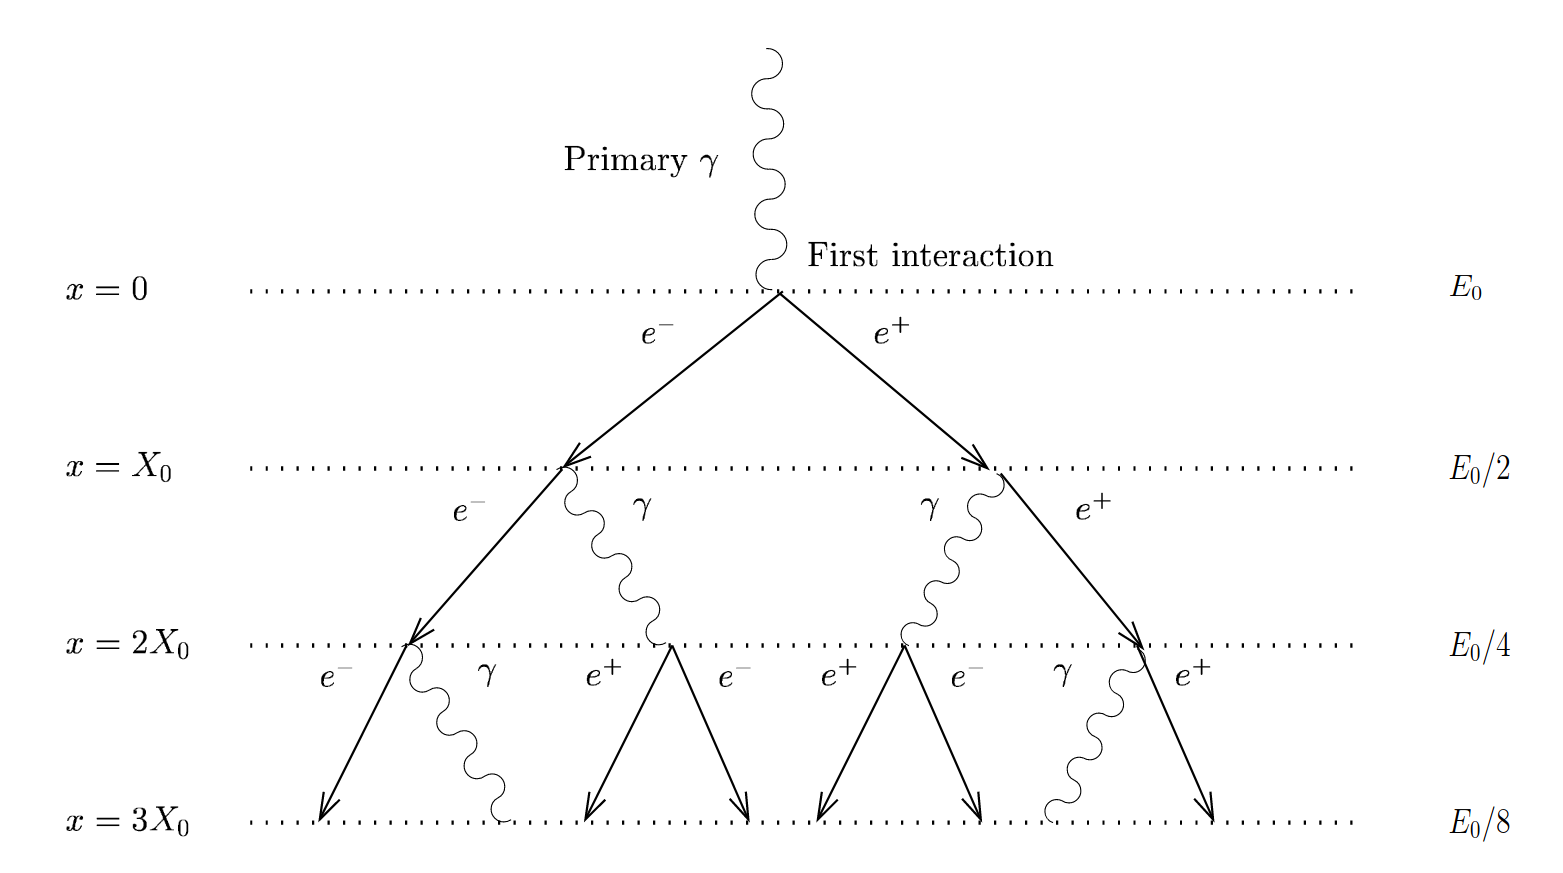
\includegraphics[width=\linewidth]{images/em_shower_illustration.png}
	\end{subfigure}%
	\begin{subfigure}{.2\textwidth}
 		\centering
		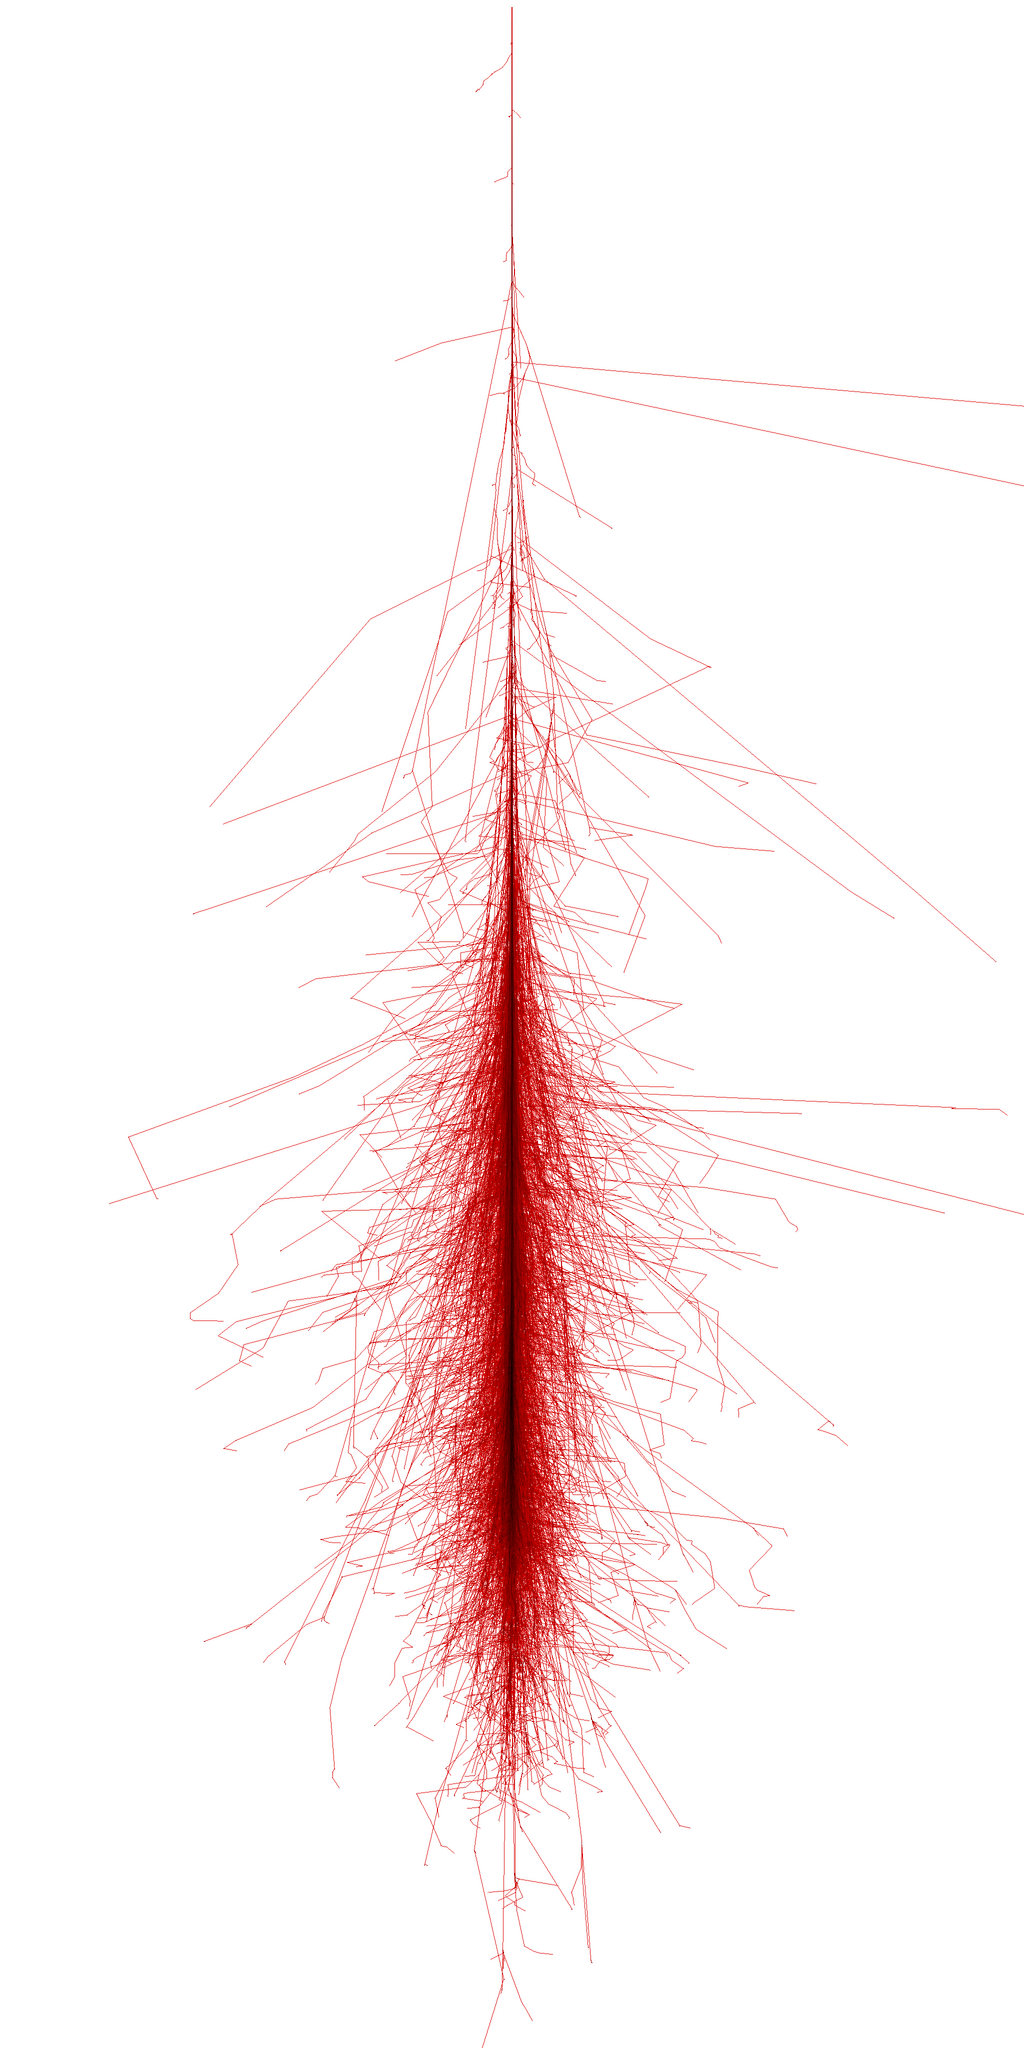
\includegraphics[width=\linewidth]{images/corsika_100gev_photon.png}
	\end{subfigure}
	\caption{
		Left: A schematic illustration of the first epochs of the 
		Bethe-Heitler shower model with equal radiation lengths for
		bremsstrahlung and pair production.
		The image is taken from an inaugural thesis 
		by Stefan Funk \cite{funk_doctor}. \\
		Right: A \SI{100}{\giga\electronvolt} gamma-shower as xz-projection, simulated with CORSIKA.
		The shower is relatively contained with only little extent perpendicular 
		to the shower direction (z-axis). The image is taken from 
		the CORSIKA-website \cite{corsika_showers}}
	\label{fig:gamma_shower}
\end{figure}

\subsection{Hadronic Showers}
Hadronic showers include all the interactions known from 
electromagnetic showers, but add nuclear interactions on top.
These lead to non-negligible additional energy losses 
and the creation of secondary hadronic particles.

Approximations are more difficult to do and monte carlo simulations 
become the only way to reasonably calculate shower behavior.

At the end of the shower a relevant portion of the particles have decayed into the 
lightest hadronic particles, pions ($\pi^0, \pi^+, \pi^-$), of which the neutral pions 
rapidly decay into photons.
This means that a part of the hadronic shower
eventually becomes an electromagnetic subshower.

Figures \ref{fig:proton_shower}
shows some of the particles generated in a hadronic shower (left)
and a \SI{100}{\giga\electronvolt} proton shower, simulated with CORSIKA (right).

\begin{figure}
	\centering
	\captionsetup{width=0.9\linewidth}
	\begin{subfigure}{.7\textwidth}
  		\centering
  		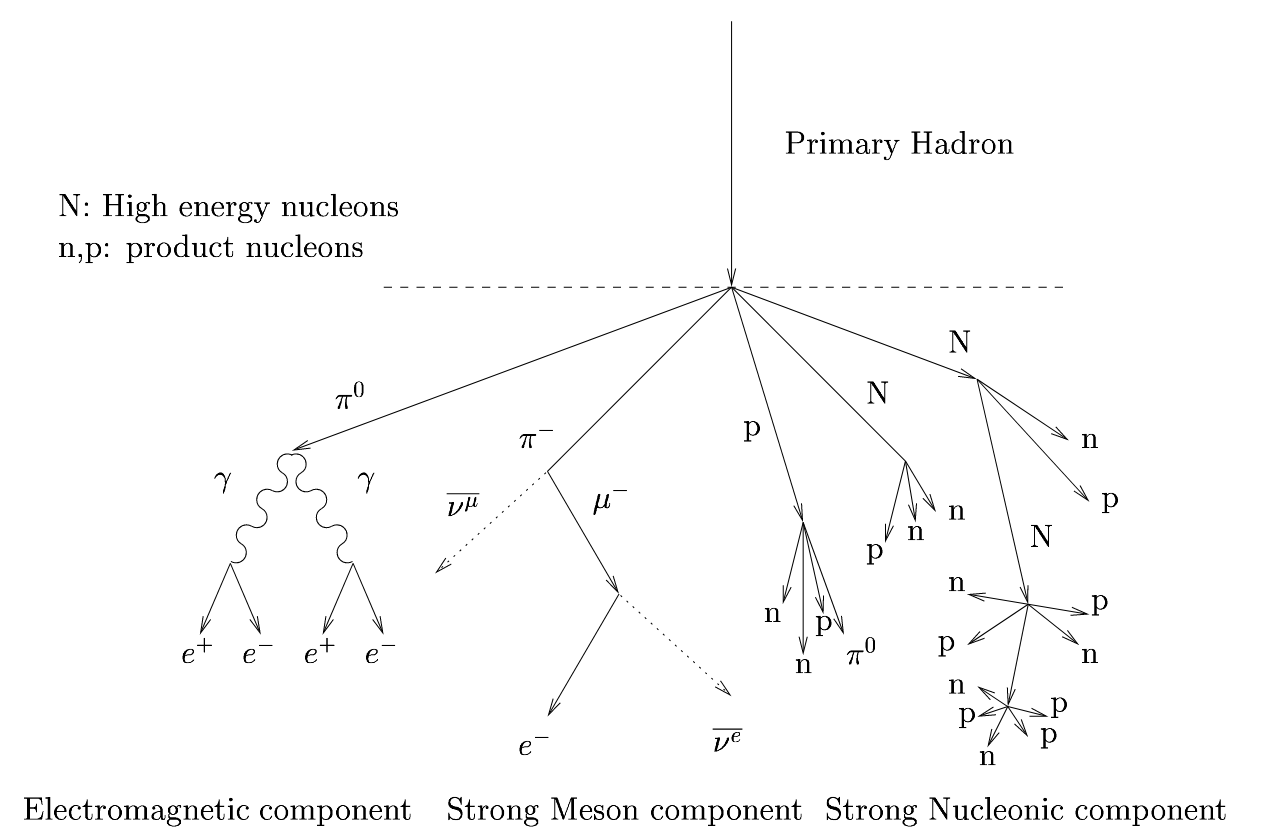
\includegraphics[width=\linewidth]{images/hadron_shower_illustration.png}
	\end{subfigure}%
	\begin{subfigure}{.2\textwidth}
 		\centering
		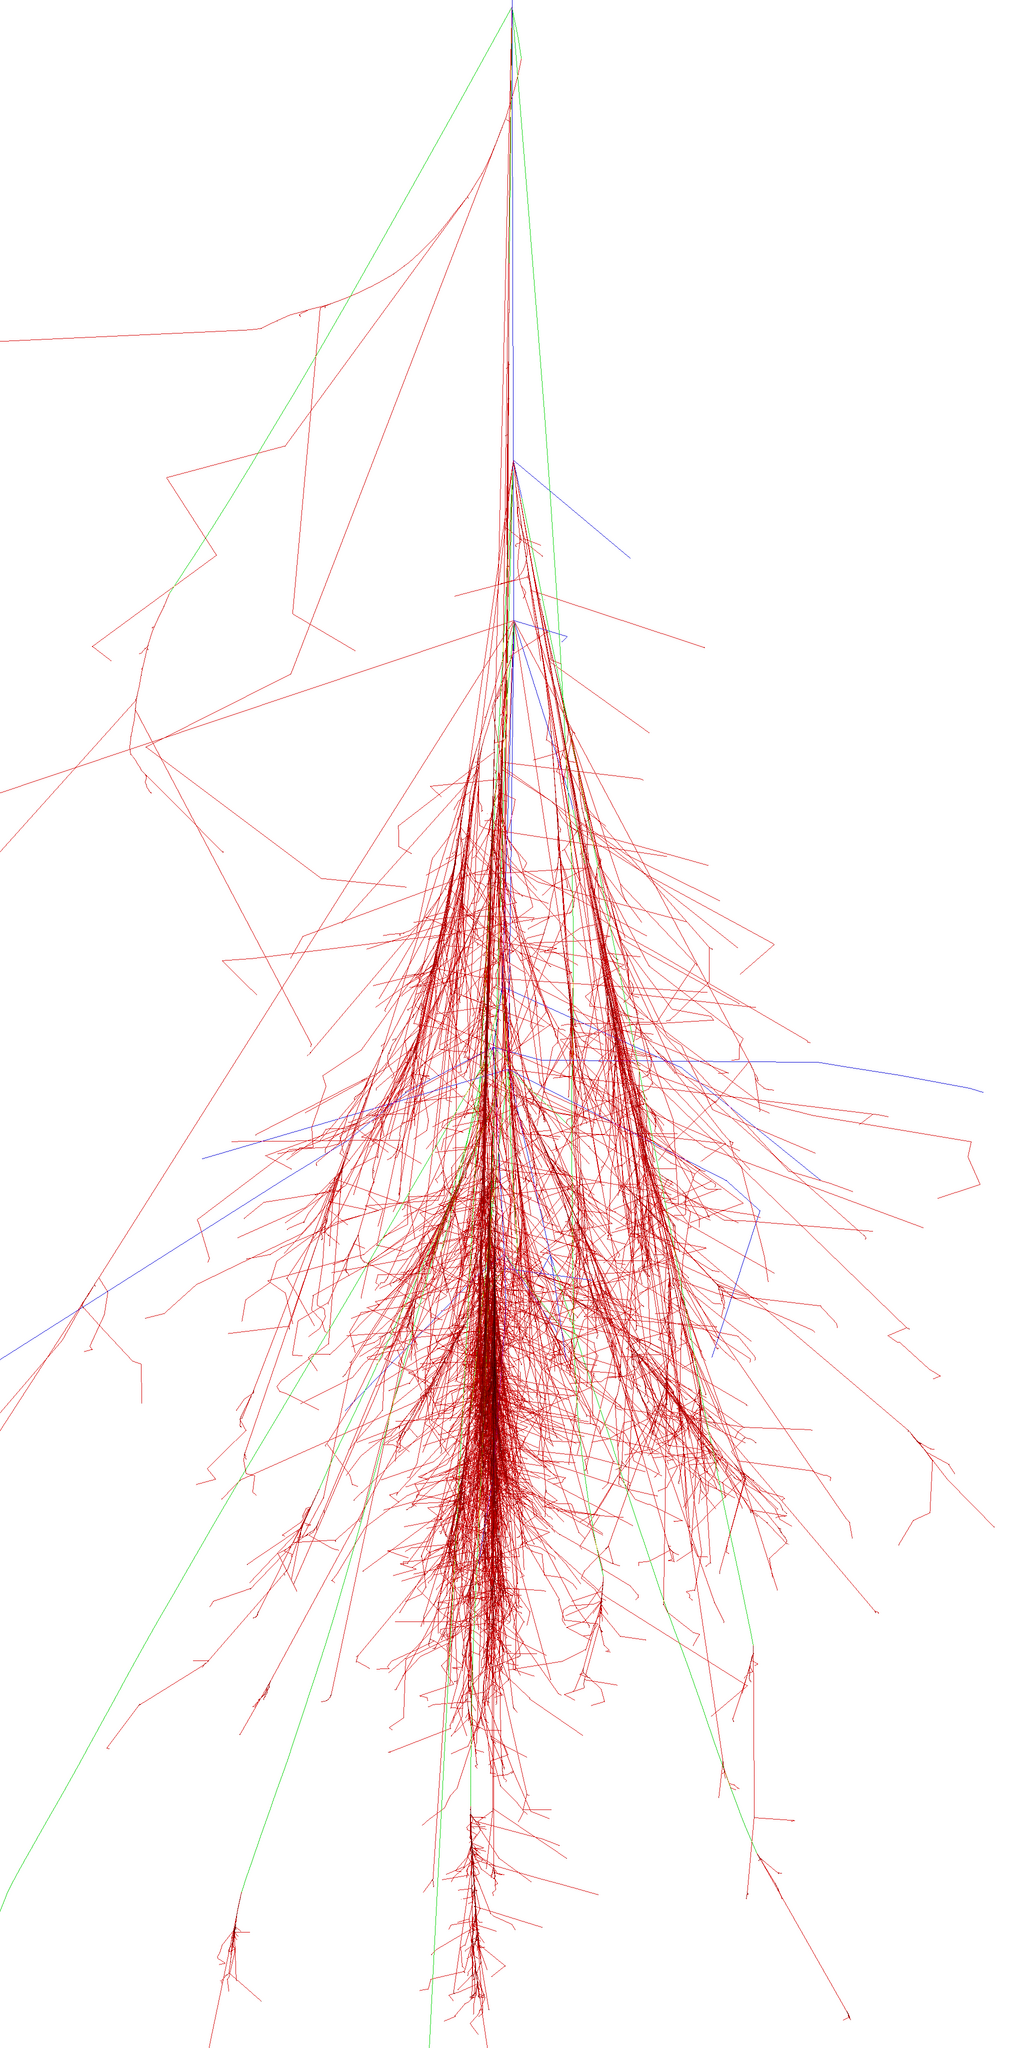
\includegraphics[width=\linewidth]{images/corsika_100gev_proton.png}
	\end{subfigure}
	\caption{
		Left: A purely qualitative,
		schematic illustration of the generation of a hadronic shower.
		It shows how the primary hadron generates different subshowers
		with vastly different particles.
		The image is taken from an inaugural thesis 
		by Stefan Funk \cite{funk_doctor}.\\
		Right: A \SI{100}{\giga\electronvolt} proton-shower as xz-projection,
		simulated with CORSIKA.
		The shower is less contained than the gamma shower of equal energy in 
		figure \ref{fig:gamma_shower}.
		Different colors indicate different particle types.
		The image is taken from 
		the CORSIKA-website \cite{corsika_showers}.}
	\label{fig:proton_shower}
\end{figure}




